\section{Introduction}
\label{sec:intro}

%\yu{1. Add more details about Taobao shopping guide assistant besides the dialog system}
An intelligent online shopping assistant
offers services such as pre-sale and after-sale inquiries, 
product recommendations, and user complaints processing,
all of which seek to give the customers better shopping experience.
\figref{fig:dialog-case} shows an example snapshot of 
such a shopping assistant. 
%\KZ{This figure is not effective. Too messy and not intuitive. I suggest we cut it. Just show a simple interface with a short conversation.}
It is a dialog module embedded in operational Taobao product search engine 
and serves as a shopping assistant on mobile Taobao.
In this example, a customer wants to buy a dress firstly. 
Then the assistant helps him
narrow down the search by getting information such as 
(\textbf{Brand}=Nike, \textbf{Color}=black).
Finally the customer changes his mind and wants to buy milk powder instead,
and this will start the next round of conversation.
%\KZ{Rephrase the following...}
%In addition to this, our system also responds to product queries. 
%All of these aim to help customers find and buy the products of their choice
%in a friendly and efficient way.

\begin{figure}[th]
	\centering
	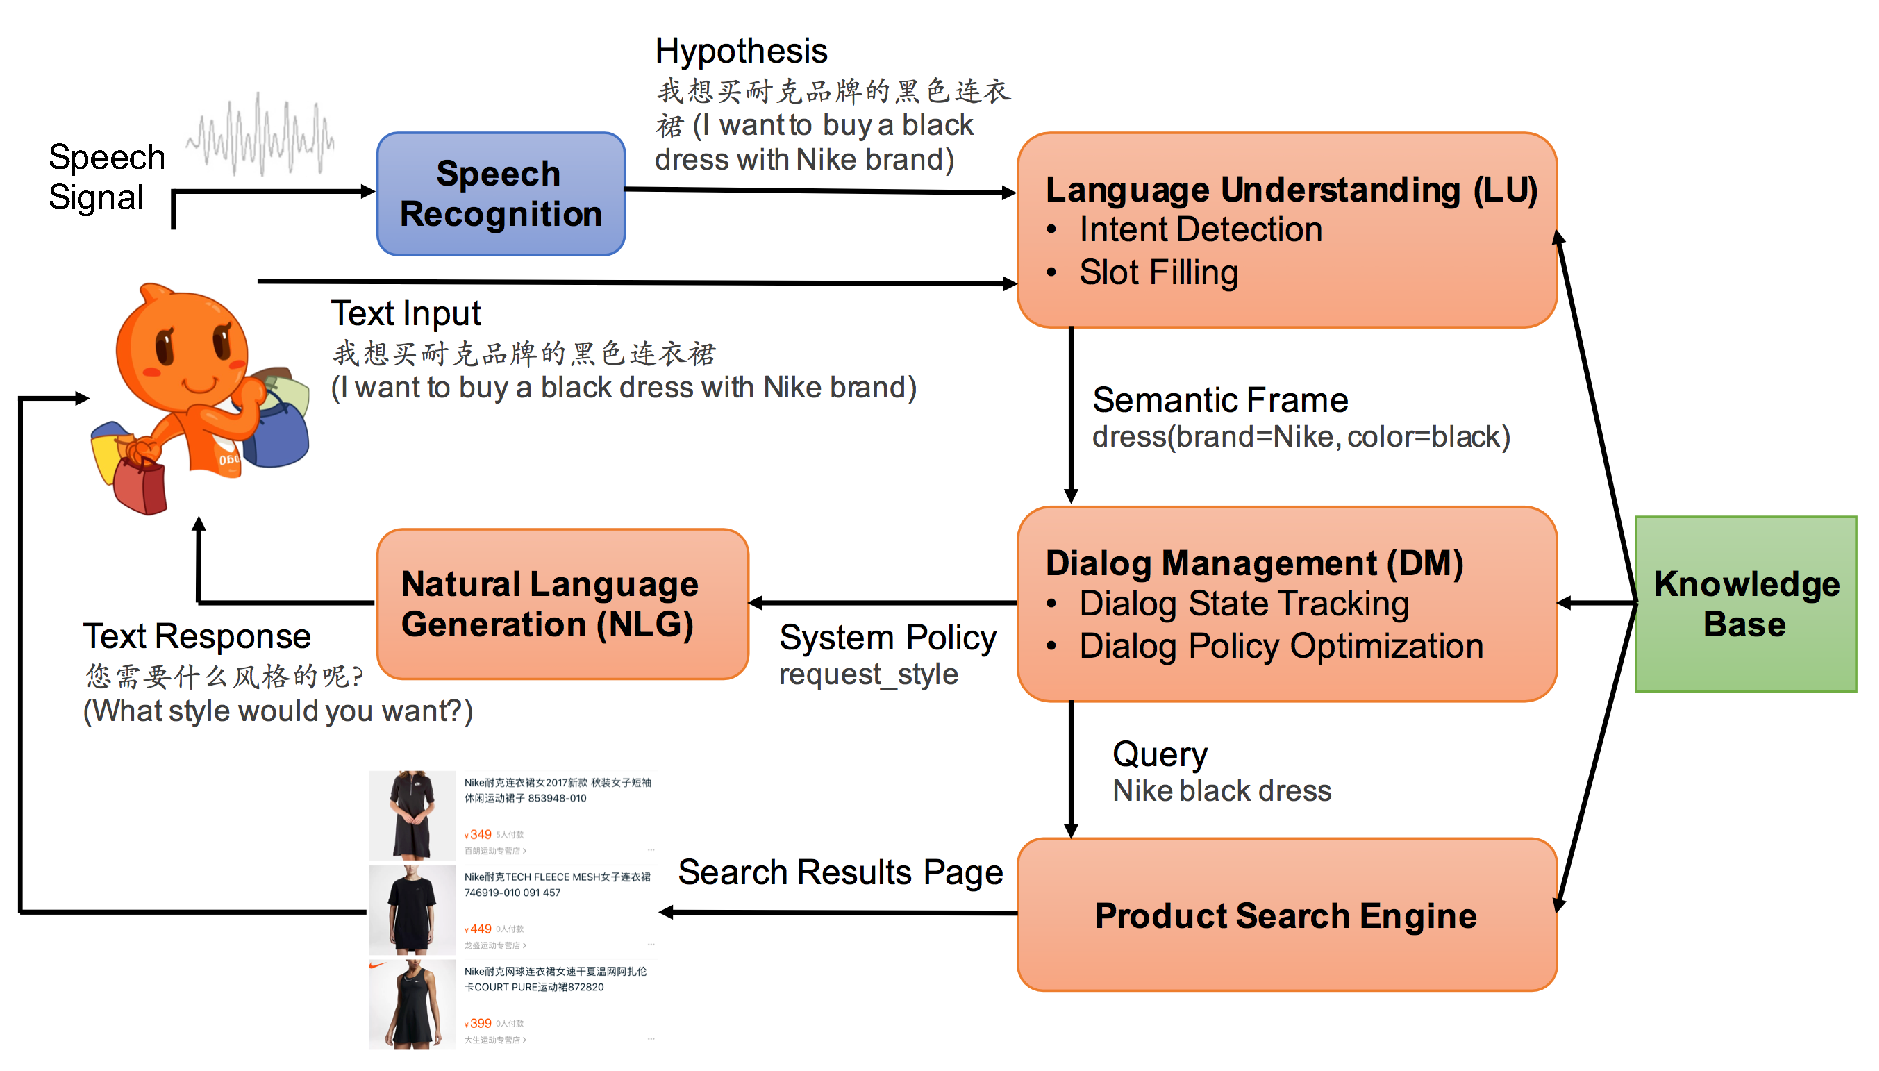
\epsfig{file=figures/dialog_system.eps, width=1.0\columnwidth}
	\caption{Pipeline framework of task-oriented dialog system for 
		shopping assistant.}
	\label{fig:dialog-system}
	%\vspace{-10pt}
\end{figure}


\begin{figure*}[th]
	\centering
	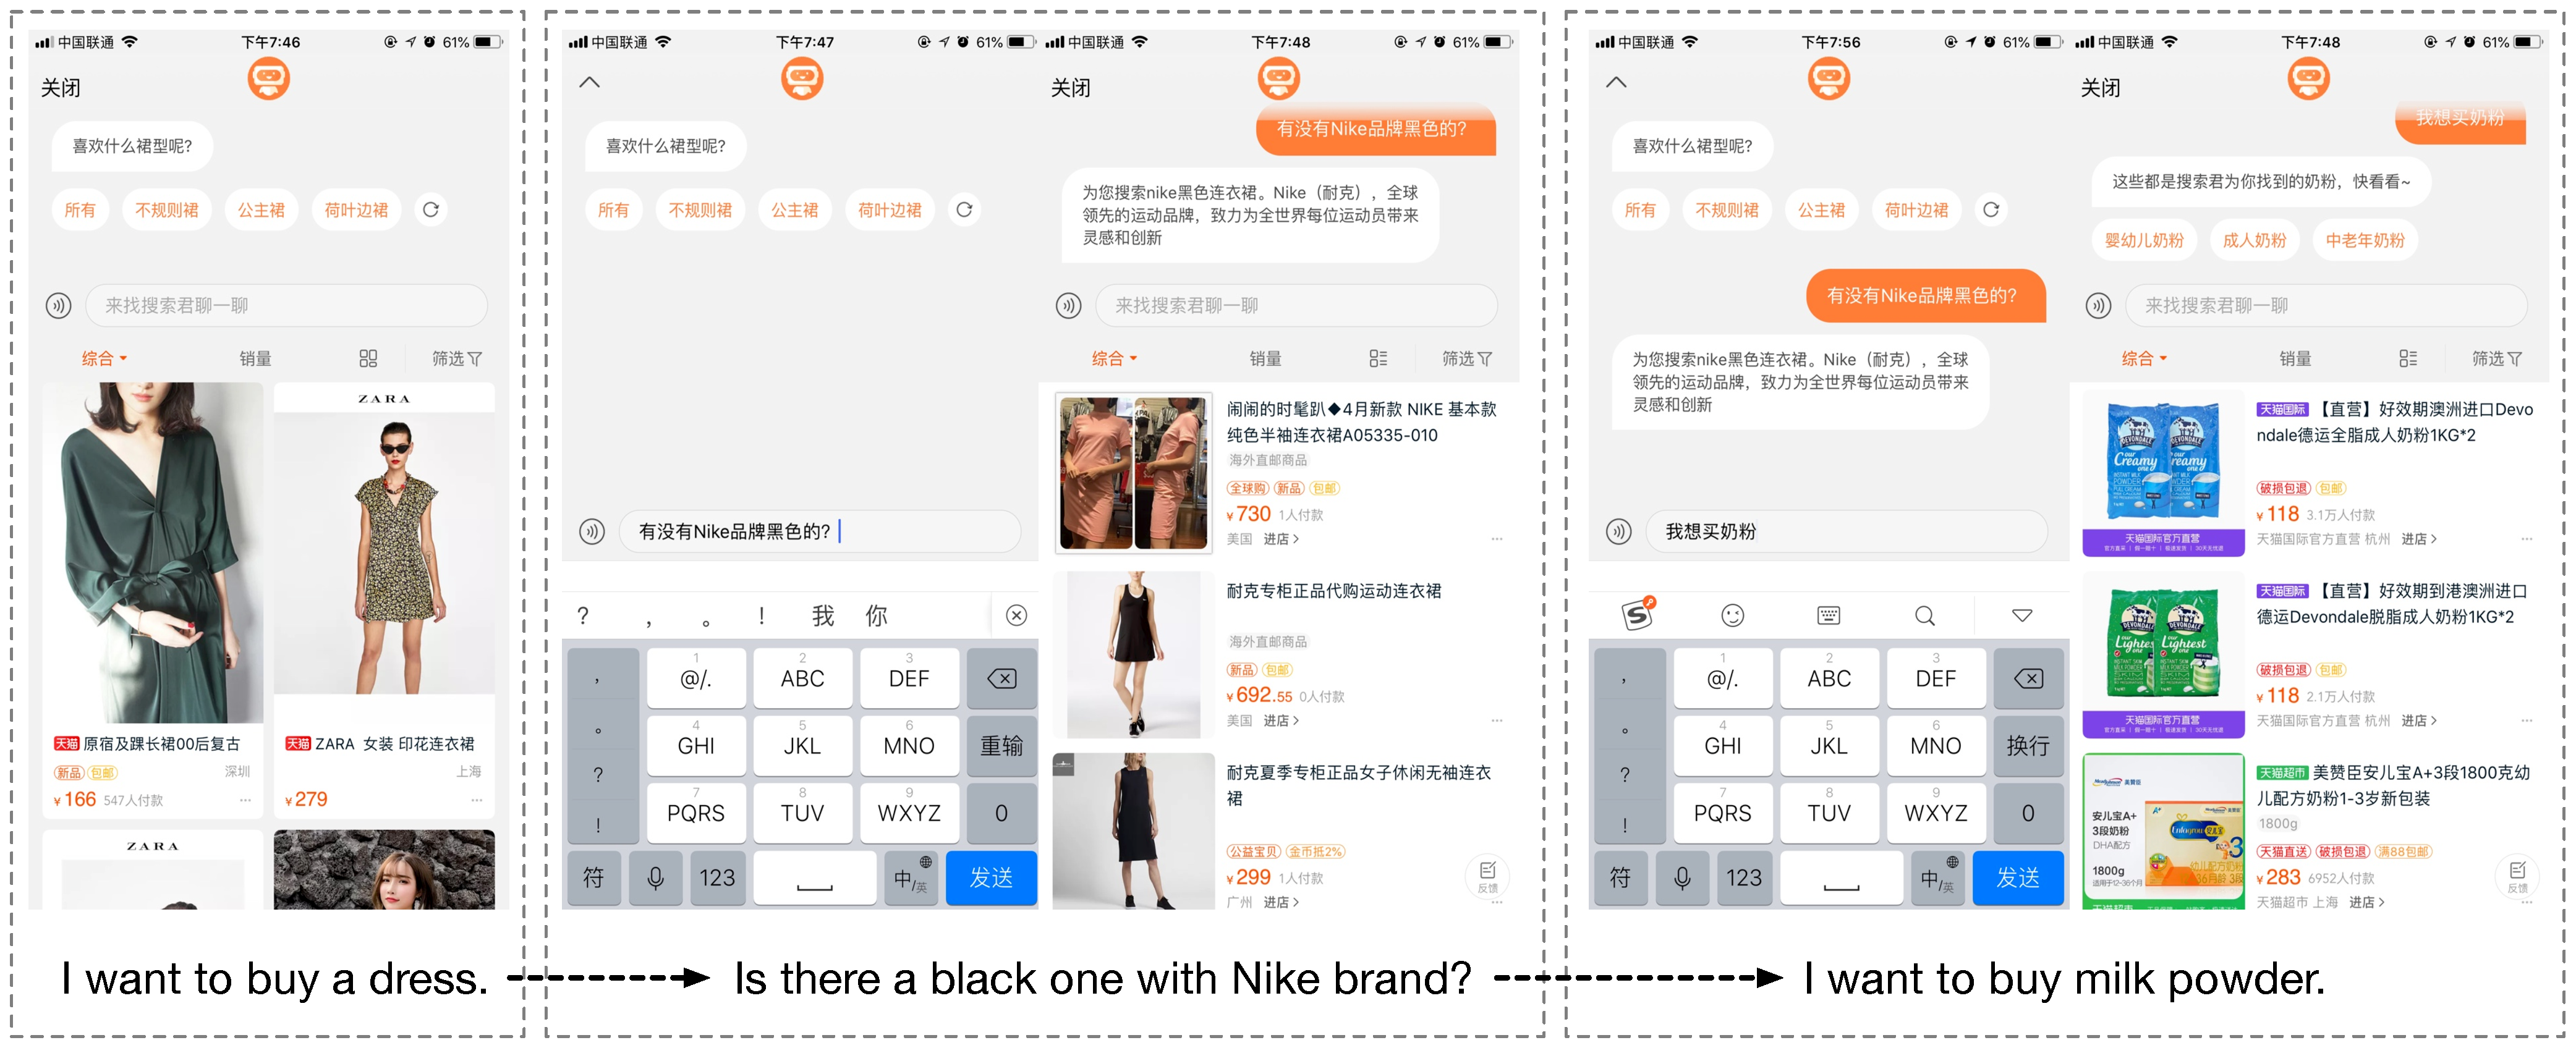
\epsfig{file=figures/dialog_case.eps, width=2.0\columnwidth}
	\caption{An example snapshot of online E-commerce shopping assistant.
	Customers will interact with our system and give sequential utterances to refine their information need or change the product intent.}
	\label{fig:dialog-case}
	%\vspace{-10pt}
\end{figure*}

%\yu{2. Dialog system, conversational search and slot filling}
The core of such assistant is a dialog system which 
has the ability to understand natural language utterances
from a user and then give natural language responses.
The general framework of such a task-oriented dialog system
is illustrated in \figref{fig:dialog-system}.
%Besides modules of dialog management (DM) and 
%natural language generation (NLG),
%the very fist step of a dialog system is
The difference between this and a traditional task-oriented dialog systems
is that it interacts with a product search engine.
%So we can also regard it as an E-commerce conversational search system.
Natural Language Understanding (NLU), which aims to 
interpret the semantic meanings conveyed by input utterances, 
is a main component in task-oriented dialog systems. 
Slot filling is a sub-problem in NLU, which identifies
the properties and their values about the task to be performed in
the dialog.
%\yu{In our E-commerce shopping guide assistant system, slot filling is not only helpful for Dialog State Tracking but also for Query Rewrite.}
%\xusheng{mentioning DST and query rewrite is a little bit strange here}


Slot filling extracts semantic constituents
by using the words of input text to fill in pre-defined slots in 
a semantic frame \cite{mesnil2015using}.
It can be regarded as sequence labeling task,
which assigns an appropriate semantic label to each word in
the given input utterance. 
In the case of E-commerce shopping, 
there are three named entity types: 
\emph{Category}, \emph{Property Key} and \emph{Property Value}.
We show a real example in \tabref{tab:slot-filling-demo}
with In/Out/Begin(IOB) scheme.
In the named entity level,
``连衣裙''\emph{(dress)} is a Category (\textbf{B-CG}/\textbf{I-CG}),
while ``品牌''\emph{(brand)} is labeled as Property Key
(\textbf{B-PK}/\textbf{I-PK}),
which is the name of one product property.
``耐克''\emph{(Nike)} and ``黑色''\emph{(black)} are labeled as Property Value
(\textbf{B-PV}/\textbf{I-PV}) since they are concrete property values.
However, mere labeling as Property Value is not good enough for the shopping
assistant.
Instead, in Slot Filling level, 
we further label ``耐克''\emph{(Nike)} as Brand Property (\textbf{B-Brand}/\textbf{I-Brand}), 
and ``黑色''\emph{(black)} as 
Color Property (\textbf{B-Color}/\textbf{I-Color}).
In the meantime, other words in the example utterance that carry 
no semantic meaning are assigned \textbf{O} label.
\begin{table*}[h]
	\centering
	\small
	\caption{A real example of slot filling in online shopping scenario.}
	\begin{tabular}{c|c|c|c|c|c|c|c|c|c|c|c|c|c}
		\toprule
		\multirow{2}{*}{Utterance} & 我 & 想 & 买 & 耐 & 克 & 品 & 牌 & 的 & 黑 & 色 & 连 & 衣 & 裙 \\
		\cmidrule{2-14}
		& \em{I} & \em{want} & \em{buy} & \multicolumn{2}{c|}{\em{Nike}} & \multicolumn{2}{c|}{\em{brand}} & $\backslash$  & \multicolumn{2}{c|}{\em{black}} & \multicolumn{3}{c}{\em{dress}} \\
		\midrule
		Slot Label & \textbf{O} & \textbf{O} & \textbf{O} & \textbf{B-Brand} & \textbf{I-Brand} & \textbf{B-PK} & \textbf{I-PK} & \textbf{O} & \textbf{B-Color} & \textbf{I-Color} & \textbf{B-CG} & \textbf{I-CG} & \textbf{I-CG} \\
		\midrule
		Named Entity Label & \textbf{O} & \textbf{O} & \textbf{O} & \textbf{B-PV} & \textbf{I-PV} & \textbf{B-PK} & \textbf{I-PK} & \textbf{O} & \textbf{B-PV} & \textbf{I-PV} & \textbf{B-CG} & \textbf{I-CG} & \textbf{I-CG} \\
		\midrule
		Segment Label & \textbf{O} & \textbf{O} & \textbf{O} & \textbf{B} & \textbf{I} & \textbf{B} & \textbf{I} & \textbf{O} & \textbf{B} & \textbf{I} & \textbf{B} & \textbf{I} & \textbf{I} \\
		\bottomrule
	\end{tabular}
	\label{tab:slot-filling-demo}
	%\vspace{-10pt}
\end{table*}

State-of-the-art sequence labeling models are typically based on 
BiLSTM-CRF \cite{huang2015bidirectional,reimers2017optimal}
and evaluated on a commonly used standard dataset ATIS \cite{price1990evaluation} in the slot filling area.
This dataset is in the domain of airline travel in America and
\tabref{tab:slot-filling-demo-atis} shows an example utterance.
However, the vocabulary size of ATIS is too small (only 572)
and slot labels are not diverse enough
since airline travel is a relatively small and specific domain,
such that recent deep learning models can achieve very high F1 scores
(nearly 0.96).
\begin{table}[h]
	\centering
	\small
	\caption{An example utterance from the ATIS dataset.}
	\begin{tabular}{c|c}
		\toprule
		Utterance & flights $|$ from $|$ Dallas $|$ to $|$ New $|$ York \\
		\midrule
		Slot Label & \makecell{\textbf{O} $|$ \textbf{O} $|$ \textbf{B-fromloc.city\_name} $|$ \textbf{O} $|$ \textbf{B-toloc.city\_name} $|$ \\ \textbf{I-toloc.city\_name}}  \\
		\bottomrule
	\end{tabular}
	\label{tab:slot-filling-demo-atis}
	%\vspace{-10pt}
\end{table}

%\KZ{I think we need to justify a bit more strongly why we need this
%new dataset.}
%\yu{In this work, we are tackling the real-world problem of slot filling for a shopping assistant on Taobao which is the largest Chinese E-commerce platform in the world.
%	It's the first attempt in the existing research for both academic and industry without any of the similar dataset.
%}

In this paper, we try to tackle a real-world slot filling problem 
for the largest Chinese E-commerce platform in the world.
The semantic  slots are much more diverse and informative than ATIS.
Thus, we create another bigger, more complex dataset
in the domain of Chinese E-commerce shopping 
assistant~\footnote{This dataset is available at \url{http://will.release.after.accepted}.}.
This dataset comes from a real world application 
and increases the difficulty for slot filling.
%This dataset comes from a real world application and the
%semantic slots are more diverse and informative than ATIS, 
%which increases the difficulty for the task.
%For example, there are 26 semantic labels in the Dress category,
%which describe different properties for a dress such as color, brand and style, while most semantic labels of ATIS 
%are related to only time and location.
For example, to describe different properties of a product for 
the purpose of utterance understanding and query rewrite,
we define large amount of informative slot labels such as color, brand, 
style, season, gender and so on.
In contrast, most semantic labels of ATIS are related to only time and location.
Furthermore, the spoken E-commerce Chinese language is more complex 
and semantically rich expression makes it harder to understand.
For example, ``红色'' and ``红'' both mean red, ``品牌'' and ``牌子'' both mean brand, ``耐克'' and ``Nike'' and ``Niky'' all mean Nike.
Whereas in ATIS, expression can be simpler, and most expressions are 
standard locations or time.

Besides, Chinese language, like many other Asian languages, are not
word segmented by nature, and word segmentation is a difficult
first step in many NLP tasks.
Without proper word segmentation, sequence labeling becomes very challenging
as the errors from segmentation will propagate.
On the other hand, more than 97\% of the chunks in ATIS data 
have only one or two words,
in which segmentation (or chunking) is not a serious problem.
Due to these reasons,
if we simply apply basic sequence labeling models,
which can be regarded as an end-to-end method,
on the Chinese E-commerce dataset,
the sentences may not be segmented correctly in the first place.
%\KZ{We need to stress more why the existing LSTM-CRF models can't handle
%the chinese e-commerce dataset.}
%\yu{Our focus and point is multi-task.}
Then the errors will propagate and the resulting slot labels will be incorrect.

%4. How Deep Cascade Multi-task learning works and the performance?
%In this paper, we employ the idea of multi-task learning
%to tackle slot filling task in Chinese E-commerce.
In this paper, we propose to employ multi-task sequence labeling model
to tackle slot filling in a novel Chinese E-commerce dialog system.
We extract two additional lower-level tasks from the slot filling task: 
{\em named entity tagging} and {\em segment tagging}.
Example labels of these two tasks 
are shown in the bottom two rows of \tabref{tab:slot-filling-demo}.
Segment tagging and named entity tagging can be regarded as 
syntactic labeling, 
while slot filling is more like semantic labeling.
Once we know the syntactic structure of an input sentence,
filling the semantic labels becomes much easier.
Compared to directly attacking slot filling,
these two low-level tasks are much easier to solve
due to fewer labels.
To this end, we propose a Deep Cascade Multi-task Learning model,
and co-train three tasks in the same framework
with a goal of optimizing the target slot filling task.
%\KZ{Earlier you said two tasks, now suddenly three tasks...}
%5. Contribution and Conclusion.

The contributions of this paper are summarized below:
\begin{itemize}
	%\itemsep0em
	\item We define a real-world problem of 
	slot filling for Chinese online shopping assistant 
	(\secref{sec:problem}), and we propose a novel deep multi-task 
	sequence labeling model (DCMTL) with cascading and 
	residual connection to solve it (\secref{sec:dcmtl}).
	\item We develop and release a Chinese E-commerce shopping assistant dataset 
	ECSA (\secref{sec:data}), which is much bigger and different from 
	the common ATIS dataset, and can be a valuable contribution to 
	dialog system research.  
	%We believe this dataset will contribute more to the future 
	%research of dialog natural language understanding.
	\item We evaluate DCMTL in both offline and online settings.
	Offline results show the model outperforms 
	several strong baseline methods by a substantial margin of $14.6\%$ on $F1$ score (\secref{sec:eval}).
	Online testing in the operational system of Taobao search shows that 
	slot filling results returned by our model achieve 130\% improvement 
	on accuracy which significantly benefits to the understanding of users' utterances (\secref{sec:case_study}). 
	%\KZ{Can we say something about the
%actual commercial impact? The accuracy seems illusive. How can you measure
%accuracy in real world interaction with users?}
%	\yu{There is no directly commercial impact, slot filling is a basic module for Query Rewrite in search area and Dialog State Tracking in dialog area.
%		So it's performance can significantly affect the user experience of the searching results. 
%	}
\end{itemize}

The rest of the paper is organized as follows:
\secref{sec:problem} provides the formal definition of slot filling problem in our study.
\secref{sec:model} describes the proposed multi-task sequence labeling architecture.
\secref{sec:data} introduces the traditional ATIS dataset and how we collect our ECSA dataset.
Then \secref{sec:implementation} gives the implementation details of our model for reproducibility.
\secref{sec:eval} presents the experimental results and analysis both on ATIS and ECSA data.
We include the detailed comparison with baseline models, ablation test for model analysis, online case study and evaluation.
\secref{sec:related} discusses some related work.
Finally \secref{sec:conclusion} concludes the paper and points out some 
future research directions.
